\section{Introduction}

Models suggest that the possibility for a larger firm to purchase a smaller firm will incentivize smaller firms to innovate. Since this buyout is voluntary, it can only mean that the entrepreneur in question gains. It is difficult to argue against the proposition that increasing the reward of an activity encourages that activity. However this possibility, does not mean the entrepreneur is more likely to invest in all projects. Quite the contrary, as the possibility increases the incentive to pursue some projects, it simultaneously decreases the incentive to pursue other projects. This paper the concept that entrepreneurs are incentivized to pursue projects which are correlated to existing firms activities.
%\textcolor{orange}{Posing the question, what is the relationship buyouts and innovation}


Empirical evidence for the link between innovation the ability to buyout is tenuous because of the difficulty in controlling for causality. There is an empirical correlation which is that industries with higher measures of innovation tend to have a more buyouts than those who don't \citep{HAU}. However there is no clear causal mechanism to describe this empirical relationship, as it may also be inferred that as innovation slows down, industry consolidation occurs \citep{COM}. 
%\textcolor{orange}{Empirical evidence}

The naive view of buyouts is simply that buyouts increase the potential payoff from innovation. We need only consider that an entrepreneur is considering the possible payoffs from his investment, ceteris paribus a probability of being bought-out, can only increase the incentive to innovate. The naive view is correct in that an extra source of payoff can only increase the upside to the entrepreneur. Even if the entrepreneur is considering numerous projects, if at least one of the projects being considered has a higher potential payoff, this can only increase the entrepreneurs incentive to innovate. This basic static logic does not necessarily generalize to long run dynamic situations. \footnote{The dynamic effect is usually interpreted as a change in industry structure in such a way that less projects become profitable in the long run \cite{bessen_maskin}}
%\textcolor{orange}{Introduces the naive view that more buyouts increase inventive to innovate}

Nevertheless the distortive effects of buyouts are not limited to being in the long run. The very option to buyout may incur immediate changes in the behavior of firms, they may change not only the \textit{absolute} payoffs of projects but also their \textit{relative} payoffs. To see why this may occur, we need only consider \textit{who} is buying out the entrepreneur. An entrepreneur has some project, this project has some value in the marketplace that is known to all. If both the entrepreneur and the firm have the same discount factor without a dynamic framework or more restrictive assumptions it is unclear why a transaction would occur\footnote{barring of course the use of a utility function}. Why would a firm pay the entrepreneur more than the entrepreneurs project \textit{isolated market value}?  There are two potential reasons why this may be the case.

%\textcolor{orange}{naive view would deny that the effect is not uniform}

Consider first the case where the project is complementary with the buyers activity if owned by the buyer. The buyers willingness to pay for the project will then be what the project is worth individually and the complementary revenue that it brings in. This would shift the incentives of the entrepreneur towards projects that are complementary with existing technology. 

Now consider the case where the entrepreneur's technology is substitutable with the buyers technology. Here the buyers willingness to pay is more complex. If the buyer has the option of shutting the project down if owned then the buyers willingness to pay does not depend on the projects value at all but depends on the buyers revenue loss if the project is not owned. \footnote{Assuming the projects market value is lower than the current activity of the buyer, if the project is worth more than the current activity then the buyer will not pay more than other buyers}

Either of these two reasons have the same result, industry convergence. Regardless of whether entrepreneur projects are complementary or substitutable with current activities. This issue is especially interesting for intellectual property, as the projects that will result due to the presence of patented ideas will be geared less towards new technological paths and more towards what existing firms will buy. In effect intellectual property can cause a sort of crowding-effect where, projects that might be very innovative and bring in millions will not be pursued because a project that can hurt a billion dollar firm by $1\%$ is has more potential upside for the entrepreneur. The inability to be complementary or be bought out can cause perfectly good projects to be thrown out. 

Since the reasoning works in the static model, it can also emerge in the dynamic one. If the different projects of the entrepreneur will both end up with the same technology but with different patterns of arrival this can equally cause firms to pursue projects of different horizons due to the possibility of being bought out. Specifically we show that projects which pass through intermediate stages of efficiency are more threatening to incumbents that projects which can more directly reach their goal. Even a technology with a lower expected value can be preferred due to the chipping away of incumbent profits. 
%\textcolor{orange}{says that the naive view is correct but its effect may not be uniform}

The paper will be presenting the case of a project which is substitutable if not owned and complementary if owned. We first give the dynamic formulation for multiple periods and arbitrary intermediate stages and then apply the model to Bertrand and Cournot competition with two periods. We will also give a brief independent version of the argument above in reduced form. 

The models presented can be interpreted in one of a few different ways. The most straightforward way is simply to say that a firm wishes to buyout another firm and the regulatory authorities either allow this or forbid this transaction. A different way is simply to say that the entrepreneur cannot be bought out because the projects are not purchasable, perhaps they are not patented or the project is simply not visible to the buyer. 

%\textcolor{orange}{three kinds of effects on incumbent depending on ownership} 

%\textcolor{orange}{Static to dynamic}

%\textcolor{orange}{The incumbent has incentive to buy the project even if it is not competitive because it ruins his margin}


%\textcolor{orange}{Gap between incumbent and entrant}


The paper is structured as follows. 
In section \ref{literature} section we will be make a few links with the literature, the model is general enough that it can be interpreted within a couple of strands. Section \ref{setup} will present the static and the dynamic versions of the model. In \ref{static} we give a brief argument to show that complementarities and substitutabilities yield the same willingness to pay, the dynamic formulation is then given in \ref{dynamic} by introducing the kind of technologies possible and some general results. The section finishes wit a brief numerical example. In section \ref{application} we apply the framework to Bertrand and Cournot competition. This is followed by a brief discussion in section \ref{discussion} before concluding. 

\section{Link to the literature}\label{literature}

Empirically it has been observed that firms which are less innovative are more likely to engage in buyouts. The work of \cite{Gerpott1995} finds that for innovation to be well absorbed by the acquirer, the firms size must not differ excessively, or said otherwise, the closer the firms are in size, the more likely they are to merge successfully. \cite{Higgins2006} find that in the pharmaceutical industry, unproductive firms are more likely to engage in acquisition strategies. This is also supported by cross industry studies such as \cite{Zhao2009}. There is also empirical work showing that companies with larger patent portfolios and low research expenditure are more likely to acquire. \cite{Bena2014}. 

%\textcolor{red}{Note that this is good for another model, buyouts are worthwhile because you get rid of patent royalty cost}.


%\textcolor{red}{An interesting note here is that actually firms that perform less well are more likely to buyout because they have lower negotiating power so they accept worse offers, but the offers payoff in the end, therefore buyouts can be interpreted as a variance strategy}

The basic theoretic framework used in this paper borrows from \cite{Cabral2003}, whose model involves two firms competing in $R\&D$ and they have an option of either choosng a high variance strategy or a low variance strategy. The general result of the model is that when a firm is lagging behind, it prefers to a high variance strategy, and when it is ahead it chooses a low variance strategy. Our results borrow from this markov chain setup but pursue different questions, mainly how does the choice between radical and incremental innovations change when the two innovations imply different payoff structures.

Our subject matter is similar to the literature on firms innovating so that they can escape competition effects(\cite{Aghion2005},\cite{Aghion2001},\cite{Aghion1997}). \cite{Gilbert2016} shows these results only hold in duopolies and not oligopolies. Other work includes \cite{Phillips2012}, where it is argued that large firms avoid engaging in $R\&D$ races. However these studies do not include different kinds of innovations, only the relative pressure to innovate depending on market positioning. 

The paper can be linked to various strands of literature, we give a brief idea of how it relates. The idea can be framed as being an application of the Coase theorem to industry structure. The question of an incumbent being harmed by an entrant can be framed within the externality framework. It is known that the Coase theorem, when transaction costs are sufficiently lows, implies an important role for extortion. A neighbor may do some activity that he would have no interest in doing because the other neighbor will be willing to pay for it. To see an interesting application of the Coase theorem with multiple possible activities see \cite{Kuechle2012}. It is also possible to interpret the results in a mechanism design framework, more specifically, auctions with allocative externalities. This literature is about preferences of ownership where agents have different utilities depending on who among the other agents owns the good, though no utility function is employed here, the results apply to other contexts for a survey of such models see, \cite{Jehiel2005}. Finally the model can be framed as being within an incomplete contract framework since there is a question of an inability for the firms to contract ex-ante. Though this is only one possible interpretation of the model, the usual reasons for uncontractibility apply, see \cite{Hart1999}.

\section{Setup}\label{setup}

\subsection{Static case: Reduced form version of the Coasian argument}\label{static}

We present the reduced form static version of the model because it illustrates that the specific complementarity or substitutability does not matter but instead it is only the \text{relative} value of owning that plays a role.  We briefly present the taxonomy under the framework and discuss why each situations may occur. 

The market profit potential of the innovation which the entrepreneur holds is given by $\pi^e$, this profit may be earned by whoever owns the entrepreneurial project. The profit of the incumbent \textit{if the innovation does not exist} is simply $\pi^i$. We denote the degree(or factor) of substitutability/complementarity \textbf{if not owned} by $\beta \in [ 0, \infty [$ and the degree of substitutability/complementarity  \textbf{if owned} by $\alpha \in [0, \infty [ $. 

The payoff if not owned is $ \beta \pi^i$. The payoff if owned is $\max\{ \pi^i, \pi^e + \alpha \pi^i   \}$. Therefore the willingness to pay for the product if  $\max\{ \pi^i, \pi^e + \alpha \pi^i   \} = \pi^i $ is: $(1-\beta) \pi^i$ and if $\max\{ \pi^i, \pi^e + \alpha \pi^i   \} = \pi^e + \alpha \pi^i $ the willingness to pay is: $\pi^e+ (\alpha-\beta) \pi^i$. The extra willingness to pay of the active firm is then simply: $(\alpha-\beta)\pi^i$. This form shows us that substitutability or complementarity do not matter for buyouts, instead it is only the \textit{relative} effects of buyouts which affect the premium the incumbent is willing to pay. Note that $\pi^i$ can then be seen as the \textit{scale} parameter. Or to express it another way, let $\zeta=1 + \frac{(\alpha-\beta)\pi^i}{\pi^e}$. If $\zeta$ is larger than 1, then the existing firm is willing to pay a premium and if the existing activity is of larger scale relative to the project, the incumbent is willing to pay a higher premium. We now briefly discuss the taxonomy of this framework. 

\textbf{Substitute}  if not owned and \textbf{Complementary} if owned implies: $\beta<1$ and $\alpha>1$. This case implies that the product will eat up the profits of the incumbent if allowed to compete with the current product but will expand profits if held together with the current activity. 

\textbf{Complementary} if not owned and \textbf{Complementary} if owned implies: $\beta>1$ and $\alpha>1$. This is just the case where whether the innovation is owned or not, the firm will benefit from it.

\textbf{Complementary} if not owned and \textbf{Neutral} if owned implies: $\beta>1$ and $\alpha=1$. Why would the project not be complementary if owned? If consumers have a specific aversion to buying things from one firm. 

\textbf{Neutral} if not owned and \textbf{Neutral} if owned implies: $\beta=1$ and $\alpha=1$. This case is simply that the entrepreneur's project is uncorrelated to the incumbents current activity.  

\textbf{Neutral} if not owned and \textbf{Complementary} if owned implies: $\beta=1$ and $\alpha>1$. If the technology is complementary this may result simply because it will make the production process more efficient or because there is a bundling effect if both goods are sold together. 

\textbf{Neutral} if not owned and \textbf{Substitute} if owned implies: $\beta=1$ and $\alpha<1$. This case would result simply in shutting down the project. It may be that if the firm markets some new product, the customers of this specific firm will flee to it. 

\textbf{Substitute} if not owned and \textbf{Neutral} if owned implies: $\beta<1$ and $\alpha=1$. Why would a project not be substitable if owned? Perhaps there is a certain way of selling the product that would interact with the incumbents product market but if the incumbent owns it, they can find a niche way to market it that allows it to be realized without eating away at their other products.


\subsection{The dynamic model}\label{dynamic}

The model is made up of an incumbent and an entrant with asymmetric initial positions. The incumbent has three possible payoffs and the entrant has two. The incumbent and entrant start out with initial technologies described by the costs, $c_i$ and $c_e$, respectively. We assume that the incumbent will initially earn the profit $\pi_i{c_i,c_e}$. The entrants earns no profit with the initial technology,$\pi_e{c_i,c_e}=0$. We say that $c_e>c_i$ to denote the efficiency of production. 

The second kind of payoffs in the model are the payoffs once the entrant catches up to the incumbent. The cost associated with this level of development is $c_{1}$. This cost is between the other two, $c_i<c_{1}<c_e$. The payoff of the incumbent when competing against this cost is lower than the payoff when competing with the less efficient entrant,$ \pi_i( c_i,c_{e}) > \pi_i( c_i, c_{e1} )$. If the incumbent were to acquire this intermediate technology, it would not use it since it is less efficient than $c_i$ so the payoff would remain unchanged. If the entrant owns the intermediate technology, the associated payoff would be weakly higher than zero, $\pi_e(c_i,c_{e1}) \geq 0$.

Finally the third kind of payoff is the payoff with the advanced technology, $c_2$. This technology is the most advanced technology available, $c_2<c_i<c_1<c_e$. Both firms would benefit from owning this technology and it represents their highest respective payoffs. 

The entrant in the model must choose what kind of innovation to engage in. The innovation is the path to the technologies above which can be achieved. There are two options, the first option passes through both stages of efficiency, we call it the \textit{sequential innovation}. The second jumps directly to the second stage of efficiency, we it the \textit{radical innovation}.  

Without loss of generality we say that the sequential innovation has no risk associated with it and does not necessarily yield profits from the first stage of efficiency. The sequential option will achieve the intermediate technology, $c_1$ after $t_1$ periods and will achieve the advanced technology, $c_2$ after $t_2$ periods. The game ends completely after $T$ periods. So if $T=t_2$ then there will only be one period where the advanced technology payoffs will be achieved. In the application to Bertrand and Cournot we will be assuming that $T=t_2=2$ and $t_1=1$ for simplicity. 

%\textcolor{orange}{Sequential innovation}

The radical innovation on the other hand will with some probability, q, give the entrant access to the advanced technology directly. So in each time period, with probability q, the firm will have cost $c_2$. If the technology fails to realize, which occurs with probability $(1-q)$ the entrant will remain at the initial technology $c_e$. If the radical innovation succeeds at any point, then the entrant will receive the advanced technology payoff until the final period, T. 

%\textcolor{orange}{Radical technology}

The difference to notice between these two methods is that the sequential innovation cannot reach the advanced payoff instantly, while the radical one can. These technologies can also be interpreted as high variance and low variance. Adoption cost of the innovations is assumed to be identical. The choice of the radical innovation and sequential technology will be represented by r and s, respectively.  

%\textcolor{orange}{The choice}

It is known that in most standard competitive frameworks, firms will want to merge because monopoly profits are higher than the sum of profits. So if bargaining is possible and credible through contracting there always exists a positive Nash Surplus that can be shared. In our framework this takes the following form: 

\begin{assumption}{Sub-additive competitive profits}
\begin{equation*}
\pi_{i}(c_{i2},c_{e}) \geq  \pi_{i}(c_{i},c_{e2}) + \pi_{e}(c_{i},c_{e2})
\end{equation*}
\begin{equation*}
\pi_{i}(c_{i},c_{e}) \geq  \pi_{i}(c_{i},c_{e1}) + \pi_{e}(c_{i},c_{e1})
\end{equation*}
\end{assumption}

%\textcolor{orange}{Buyout is always done in Bertrand competition}

We assume that firms do not have a preference for future or negative profits. Though there is no \text{preference} for present profits, the interpretation of the model can be interpreted as discounting because firms naturally will prefer one innovation over the other because of their time structure. 

We now specify the timing of the model. The first decision that occurs is the innovation decision of the entrant, the choice between sequential or radical innovation. If no buyouts are allowed, then the payoff streams occur. If there are buyouts, then after the choice of innovation occurs, negotiation occurs between the entrant and the incumbent for a buyout, after which the buyout payoff streams are realized.

Notice that if it were possible for the buyout to materialize before the choice of innovation(ex-ante) this would result in simply the innovation with the highest expected payoff to happen. This could come about if the entrant was able to credibly signal to the incumbent that the incumbent is capable of undertaking the investment. An implication of an ex-ante buyout is that the incumbent pays a weakly higher amount for the innovation. It is easiest to see in the case where the entrant chooses an innovation which does not maximize market payoffs. This would be the blackmail case where the firm entrant can use the threat of substitutability to make the incumbent pay for the externalities imposed by the entrant. Note that if the radical innovation is bought, this does not guarantee the realization of the technology. 

%\textcolor{red}{Assume both technological steps improve cost by the same amount}
\subsubsection{Sequential}

The sequential innovation will give the intermediate technology after $t_1$ periods and the advanced technology after $t_2$ periods. Therefore the total profit of the entrant is simply: 

\begin{equation*}
\Pi_{es} = \pi_e(c_i,c_{i1}) (t_2-t_1) +\pi_e(c_i,c_{e2})(T+1-t_2)
\end{equation*}

The payoff of the incumbent is similar except that there is an additional stream of payments for the first $t_1$ periods before the entrant is competitive enough to compete. 

\begin{equation*}
\Pi_{is} = \pi_i(c_i,c_{e})t_1+\pi_i(c_i,c_{i1}) (t_2-t_1)+\pi_i(c_i,c_{e2})(T+1-t_2)
\end{equation*}

The merger profit of the incumbent will ignore the first $t_1$ periods because the intermediate technology is not an improvement on the initial technology. There is no direct value added to the incumbent payoff from variations in $t_1$. As we will see $t_1$ does matter for the effect it has on the bargaining disagreement payoff of the entrant. The merger profit is simply given by: 

\begin{equation*}
\Pi_{s}^m= \pi_i(c_i,c_{e}) t_2+\pi_i(c_{i2},c_e)(T+1-t_2)
\end{equation*}

From the two payoffs of the entrant we can deduce the willingness to pay for the sequential innovation: 

\begin{align*}
WTP=\Pi_{s}^m-\Pi_{is} = (\pi_i(c_i,c_{e})-\pi_i(c_i,c_{i1}))(t_2-t_1)+(\pi_i(c_{i2},c_e)-\pi_i(c_{i},c_{e2}))(T+1-t_2) \\
\end{align*}

We need only subtract the payoff of the entrant from the willingness to pay to have the bargaining surplus, that is the value added from merging:

\begin{align*}
S_s= (\pi_i(c_i,c_{e})-\pi_i(c_i,c_{i1})-\pi_e(c_i,c_{i1}))(t_2-t_1)+(\pi_i(c_{i2},c_e)-\pi_i(c_{i},c_{e2})-\pi_e(c_{i},c_{e2}))(T+1-t_2) 
\end{align*}

The surplus will be split based on bargaining power $\omega \in [0,1]$, where if $\omega = 1$, all the surplus is taken by the entrant and if $\omega = 0$, all surplus is taken by the incumbent. The bargaining payoff of the entrant is therefore:

\begin{align*}
B_{es}(\omega) &= \Pi_{es}+ \omega S_s \\
%%%%%%%%%%%%%%%%%%%%%%%%%%%%%%%%%%%%%
&=(\omega(\pi_i(c_i,c_{e})-\pi_i(c_i,c_{i1}))+(1-\omega)\pi_e(c_i,c_{i1}))(t_2-t_1) \\
%%%%%%%%%%%%%%%%%%%%%%%%%%%%%%%%%%%%%
&+(\omega(\pi_i(c_{i2},c_e)- \pi_i(c_{i},c_{e2}))+(1-\omega)\pi_e(c_{i},c_{e2}))(T+1-t_2) \\
%%%%%%%%%%%%%%%%%%%%%%%%%%%%%%%%%%%%%
B_{is}(\omega) &= \Pi_{is}+(1-\omega)S_s \\
%%%%%%%%%%%%%%%%%%%%%%%%%%%%%%%%%%%%%
& =\pi_i(c_i,c_{e})t_1 \\
%%%%%%%%%%%%%%%%%%%%%%%%%%%%%%%%%%%%%
&+(\omega \pi_i(c_i,c_{i1})+(1-\omega)(\pi_i(c_i,c_{e})-\pi_e(c_i,c_{i1})))(t_2-t_1)
%%%%%%%%%%%%%%%%%%%%%%%%%%%%%%%%%%%%%
\\&+(\omega \pi_i(c_i,c_{e2})+(1-\omega)(\pi_i(c_{i2},c_e)-\pi_e(c_{i},c_{e2})))(T+1-t_2)
\end{align*}

Note that the bargaining payoff of the entrant is increasing in $T$ and decreasing in $t_1$. 

\subsubsection{Radical}

In the radical innovation, the probability that the entrant receives $T$ flows of advanced technology payoffs is given by q. Similarly the probability of receiving $T-1$ is $q(1-q)$, of $T-2$, $q(1-q)^2$, etc. Therefore the general payoff for the entrant is given by:

\begin{align*}
\Pi_{er} & = 
\pi_{e}(c_i,c_{e2}) q \sum_{i=1}^{T} (1-q)^{i-1} (T+1-i) \\
%%%%%%%%%%%%%%%%%%%%%%%%%%%%%%%%%%%
&= \pi_{e}(c_i,c_{e2}) \left( T - \frac{(1-q)}{q} \left( 1-(1-q)^T \right) \right) \\
\end{align*}

The incumbent payoff will take a similar form to the entrant but will receive non-zero payoffs regardless of the realization. Or to express this in another way, the expected number of payoffs is given by $T$. This means that we need only subtract the previous expected number of streams from T to receive the expected number of streams with the initial technology. This is given below: 

\begin{align*}
\Pi_{ir} =& \pi_{i}(c_i,c_{e2}) \underbrace{q \sum_{i=1}^{T} (1-q)^{i-1} (T+1-i)}_{\text{Expected number of } \pi_{i}(c_i,c_{e2})}+ \pi_i(c_i,c_e) \underbrace{ (T-q \sum_{i=1}^{T} (1-q)^{T-i} i)}_{\text{Expected number of } \pi_{i}(c_i,c_{e})}
\\
=& \pi_{i}(c_i,c_{e2}) q \sum_{i=1}^{T} (1-q)^{T-i} i + \pi_i(c_i,c_e)  \sum_{i=1}^T (T-q \sum_{i=1}^{T} (1-q)^{T-i} i)
\\ =& \pi_{i}(c_i,c_{e2})q \sum_{i=1}^{T} (1-q)^{i-1} (T+1-i)+ \pi_i(c_i,c_e) (T-q \sum_{i=1}^{T} (1-q)^{T-i} i)
\\ =&\pi_{i}(c_i,c_{e2}) \left( T - \frac{(1-q)}{q} \left( 1-(1-q)^T \right) \right)
+\pi_i(c_i,c_e) \frac{(1-q)}{q} \left( 1-(1-q)^T \right) \\
\end{align*}

So with the buyout, the merger payoff of the incumbent is given by a similar expression, where the only difference is that the technology $c_2$ is owned by the incumbent instead of the entrant. 

\begin{align*}
\Pi^m_r = \pi_{i}(c_{i2},c_{e}) \left( T - \frac{(1-q)}{q} \left( 1-(1-q)^T \right) \right)
+\pi_i(c_i,c_e) \frac{(1-q)}{q} \left( 1-(1-q)^T \right)
\end{align*}

As before, the corresponding willingness to pay of the incumbent and Nash surplus to be shared are given by: 

\begin{align*}
WTP_r &= (\pi_{i}(c_{i2},c_{e})-\pi_{i}(c_{i},c_{e2})) \left( T - \frac{(1-q)}{q} \left( 1-(1-q)^T \right) \right) \\
S_r &= (\pi_{i}(c_{i2},c_{e})-\pi_{i}(c_{i},c_{e2})-\pi_{e}(c_{i},c_{e2})) \left( T - \frac{(1-q)}{q} \left( 1-(1-q)^T \right) \right)
\end{align*}

The bargaining payoff is then:

\begin{align*}
B_{er}(\omega) &= \Pi_{er}+\omega S_r \\
&= \left(\omega\pi_{i}(c_{i2},c_{e})-\omega \pi_{i}(c_{i},c_{e2})+(1-\omega)\pi_{e}(c_{i},c_{e2}) \right) \left( T - \frac{(1-q)}{q} \left( 1-(1-q)^T \right) \right) \\
B_{ir}(\omega) &=\pi_{i}(c_i,c_{e2}) \left( T - \frac{(1-q)}{q} \left( 1-(1-q)^T \right) \right)
+\pi_i(c_i,c_e) \frac{(1-q)}{q} \left( 1-(1-q)^T \right)
\\ &+(1-\omega)(\pi_{i}(c_{i2},c_{e})-\pi_{i}(c_{i},c_{e2})-\pi_{e}(c_{i},c_{e2})) \left( T - \frac{(1-q)}{q} \left( 1-(1-q)^T \right) \right) \\
&=\pi_i(c_i,c_e) \frac{(1-q)}{q} \left( 1-(1-q)^T \right)
\\ &+(\omega \pi_i(c_i,c_{e2})+(1-\omega)(\pi_{i}(c_{i2},c_{e})-\pi_{e}(c_{i},c_{e2}))) \left( T - \frac{(1-q)}{q} \left( 1-(1-q)^T \right) \right)
\end{align*}

\subsubsection{The distortion of buyouts}

We now show the general result for the distortion of incentives. First note that the entrant will choose the radical innovation over the sequential innovation purely on the expected values of the entrants payoffs. We denote the condition for preferring the radical innovation as as $\Delta \Pi$, it's general form is the following: 

\begin{align*}
\Pi_{er}  &> \Pi_{es}   \\
\pi_{e}(c_i,c_{e2}) \left( T - \frac{(1-q)}{q} \left( 1-(1-q)^T \right) \right) - \pi_e(c_i,c_{i1}) (t_2-t_1) -\pi_e(c_i,c_{e2})(T+1-t_2) &> 0 \\
\pi_{e}(c_i,c_{e2}) \left( t_2 -1- \frac{(1-q)}{q} \left( 1-(1-q)^T \right) \right) - \pi_e(c_i,c_{i1}) (t_2-t_1)  &> 0 \\
\leftrightarrow
\Delta \Pi &> 0
\end{align*}

$\Delta \Pi$ is clearly increasing in q and $t_2$, note especially that the effect of $t_2$ is two fold. The first appearance is the loss of relative profitability relative to the radical project, whilst the second term is the absolute loss in expected value of the sequential innovation. 

\begin{proposition}
As the time horizon increase, the preference for the radical innovation decreases. The decrease is slower for higher increments. 
\end{proposition}

\begin{proof}
\text{The first order condition with respect to T is}
\begin{align*}
\frac{\partial \Delta \Pi}{\partial T}=\frac{\pi_{e}(c_i,c_{e2})}{q} (1-q)^{T+1} \log[1-q] \\
\text{The second condition with respect to T is} \\
\frac{\partial \Delta^2 \Pi}{\partial T^2} = \frac{\pi_{e}(c_i,c_{e2})}{q} (1-q)^{T+1} \log[1-q]^2
\end{align*}
\text{Both of which are negative}
\end{proof}

If buyouts are allowed, the entrant will then compare the bargaining payoffs instead of the market payoffs: 

\begin{align*}
B_{er}(\omega) > B_{es}(\omega) \\
\leftrightarrow \\
%%%%%%%%%%%%%%%%%%%%%%%%%%%%%%%%%%%%%
\left(\omega\pi_{i}(c_{i2},c_{e})-\omega \pi_{i}(c_{i},c_{e2})+(1-\omega)\pi_{e}(c_{i},c_{e2}) \right) \left( T - \frac{(1-q)}{q} \left( 1-(1-q)^T \right) \right)> \\ 
%%%%%%%%%%%%%%%%%%%%%%%%%%%%%%%%%%%%%
(\omega(\pi_i(c_i,c_{e})-\pi_i(c_i,c_{i1}))+(1-\omega)\pi_e(c_i,c_{i1}))(t_2-t_1) \\
%%%%%%%%%%%%%%%%%%%%%%%%%%%%%%%%%%%%%
+(\omega(\pi_i(c_{i2},c_e)- \pi_i(c_{i},c_{e2}))+(1-\omega)\pi_e(c_{i},c_{e2}))(T+1-t_2) \\
%%%%%%%%%%%%%%%%%%%%%%%%%%%%%%%%%%%%%
\leftrightarrow \\
\left(\omega (\pi_{i}(c_{i2},c_{e})- \pi_{i}(c_{i},c_{e2}))+(1-\omega)\pi_{e}(c_{i},c_{e2}) \right) \left( t_2-1 - \frac{(1-q)}{q} \left( 1-(1-q)^T \right) \right)  \\
%%%%%%%%%%%%%%%%%%%%%%%%%%%%%%%%%%%%%
-(\omega(\pi_i(c_i,c_{e})-\pi_i(c_i,c_{i1}))+(1-\omega)\pi_e(c_i,c_{i1}))(t_2-t_1)>0 \\
\leftrightarrow
\Delta B > 0
\end{align*}

If the entrant has no bargaining power, the incentives with and without buyout are identical, $(\omega=0 \rightarrow \Delta B = \Delta \Pi)$. This leads us to the main proposition of the paper which is that the excess incentive of pursuing sequential innovation. 

\begin{proposition} \label{excessincentive}
The excess incentive required for the entrant to pursue the radical innovation when there are buyouts is given by: 
\begin{align*}
\omega \left(  \pi_{i}(c_{i2},c_{e})- \pi_{i}(c_{i},c_{e2})-\pi_{e}(c_{i},c_{e2})  \left( t_2-1  - \frac{(1-q)}{q} \left( 1-(1-q)^T \right) \right) \right. \\
%%%%%%%%%%%%%%%%%%%%%%%%%%%%%%%%%%%%%
-\left.(\pi_i(c_i,c_{e})-\pi_i(c_i,c_{e1})-\pi_e(c_i,c_{e1}))(t_2-t_1) \right)  >0 \\
\end{align*}
\end{proposition}


If $\Delta B$ is larger than $\Delta \Pi$, this means that the requirements for the radical innovation to be preferred are more stringent in the buyout case than the non-buyout case. The buyout option will always benefit the entrant because by definition the entrant can always just ignore that option. However the buyout option does not always benefit the incumbent. 

There are four cases to consider for the incumbent to prefer buyouts. Since the incumbent in the real world would have a willingness to pay for the different regimes it is worth exploring under what cases the buyouts would be preferred. If the buyout affects preferences it is always in favor of the sequential innovation, which means that if it affects preferences it means that the entrant will pursue the sequential innovation. We can dismiss the case where the buyout has no effect on preferences or on the decision to enter, in such a case the classic analysis holds, the only effects of buyouts is to increase the payoff of both the incumbent and the entrant. \newline


\subsubsection{Case 1: Does not affect preferences, but affects decision to enter} \label{case:decision}
In case two, the entrant would not have entered at all but due to the incentive effect of the buyout the entrant has instead decided to enter. To evaluate this case we need only note that without the buyout, the incumbent would receive T flows of $\pi_i(c_i,c_e)$. The incumbent will therefore prefer the buyout if the flow is inferior to the bargaining payoff: 

\begin{align*}
B_{is}(\omega)&>T \pi_i(c_i,c_e) \\
& \leftrightarrow (\omega \pi_i(c_i,c_{i1})+(1-\omega)(\pi_i(c_i,c_{e})-\pi_e(c_i,c_{i1})))(t_2-t_1) \\
%%%%%%%%%%%%%%%%%%%%%%%%%%%%%%%%%%%%%
&+(\omega \pi_i(c_i,c_{e2})+(1-\omega)(\pi_i(c_{i2},c_e)-\pi_e(c_{i},c_{e2})))(T+1-t_2)
%%%%%%%%%%%%%%%%%%%%%%%%%%%%%%%%%%%%%
\\&- \pi(c_i,c_e)(T-t_1)>0 \\
B_{ir}(\omega)&>T \pi_i(c_i,c_e) \\
& \leftrightarrow (\omega \pi_i(c_i,c_{e2})+(1-\omega)(\pi_{i}(c_{i2},c_{e})-\pi_{e}(c_{i},c_{e2}))-\pi_i(c_i,c_e)) \left( T - \frac{(1-q)}{q} \left( 1-(1-q)^T \right) \right)>0 \\
&\rightarrow 
(\omega \pi_i(c_i,c_{e2})+(1-\omega)(\pi_{i}(c_{i2},c_{e})-\pi_{e}(c_{i},c_{e2}))-\pi_i(c_i,c_e))>0
\end{align*}


\subsubsection{Case 2: Affects preferences but not decision to enter} \label{case:preference}

Since the entrant would have entered anyway but the only thing that has changed is the choice of innovation this is simply the difference in payoff between the bargaining payoff in the sequential innovation and the market payoff with the radical innovation. 

\begin{align*}
&B_{is}(\omega)>\Pi_{ir}
\\
%%%%%%%%%%%%%%%%%%%%%%%%%%%%%%%%%%%%%
& \leftrightarrow \pi_i(c_i,c_{e})t_1 
%%%%%%%%%%%%%%%%%%%%%%%%%%%%%%%%%%%%%
+(\omega \pi_i(c_i,c_{i1})+(1-\omega)(\pi_i(c_i,c_{e})-\pi_e(c_i,c_{i1})))(t_2-t_1)
%%%%%%%%%%%%%%%%%%%%%%%%%%%%%%%%%%%%%
\\&+(\omega \pi_i(c_i,c_{e2})+(1-\omega)(\pi_i(c_{i2},c_e)-\pi_e(c_{i},c_{e2})))(T+1-t_2)  \\
%%%%%%%%%%%%%%%%%%%%%%%%%%%%%%%%%%%%%
&> \pi_{i}(c_i,c_{e2}) \left( T - \frac{(1-q)}{q} \left( 1-(1-q)^T \right) \right)
+\pi_i(c_i,c_e) \frac{(1-q)}{q} \left( 1-(1-q)^T \right) \\
%%%%%%%%%%%%%%%%%%%%%%%%%%%%%%%%%%%%%%
\leftrightarrow &\pi_i(c_i,c_e)(t_2 -\omega(t_2-t_1)-\frac{(1-q)}{q} \left( 1-(1-q)^T \right)) 
%%%%%%%%%%%%%%%%%%%%%%%%%%%%%%%%%%%%%%
+(\omega \pi_i(c_i,c_{i1})-(1-\omega)\pi_e(c_i,c_{i1}))(t_2-t_1) \\
%%%%%%%%%%%%%%%%%%%%%%%%%%%%%%%%%%%%%%
& +(1-\omega)(\pi_i(c_{i2},c_e)-\pi_e(c_{i},c_{e2}))(T+1-t_2) \\
%%%%%%%%%%%%%%%%%%%%%%%%%%%%%%%%%%%%%%
&+ \pi_i(c_{i},c_{e2})\left(\omega(T+1-t_2)-T+\frac{(1-q)}{q} \left( 1-(1-q)^T \right)\right)
> 0
\end{align*}

\subsubsection{Case 3: Affects preferences and decision to enter}\label{case:both}

If it affects both the preference and the decision to enter this means that the incumbent will receive the non-competitive flows for T periods or necessarily be bargaining with a sequential innovation entrant. The condition is the same as in case \ref{case:decision}, $ B_{is}(\omega)>T \pi_i(c_i,c_e)$.

\subsection{Numerical example with two time periods}

Suppose that the profit of the entrant with the best technology is given by, $40$. The profit of the incumbent with best technology is given by $100$. Additionally, let the profit of the incumbent when competing with an intermediate technology be $20$, whilst the profit of the incumbent with the initial technology is: $=80$. Finally, we assume a simple Nash bargaining solution where firms have equal bargaining power, $\omega = .5$ and that the radical innovation has a $50$\% chance of succeeding. 

We first do the case where there are no buyouts. If no buyouts do occur and the entrant chooses the sequential innovation then the entrant will simply earn, $40$, which will only be realized in the second period. If the entrant chooses the radical innovation the payoff will simply be $.5(40+40)+(.5)^2(40)=50$. Since $50>40$, if no buyout occurs the radical innovation will be chosen. 

If buyouts do occur then the incentives change. The Nash surplus for the sequential innovation is, $NS_s = 100+80-20-40=120$. Therefore the payoff of the entrant after bargaining is $40+\frac{1}{2}(120)=100$. The radical innovation surplus is similarly $NS_r = .5(200)+(.5)^2 180+(.5)^2 160-(.5)^2 80-(.5)^2-50=75$. Therefore the payoff after bargaining $50+\frac{1}{2}(75)=87.5$ so the entrant pursues the sequential innovation. 

\section{Applications:}\label{application}

To clarify ideas and develop our intuition we now apply the general concept to Bertrand and Cournot competition. Without loss of generality we assume that both $\pi_i(c_i,c_e)$ and
$\pi_i(c_{i2},c_e)$ are monopoly profits. That is, the gap between the technologies is sufficiently large that the entrant simply sets the monopoly price. We also assume a simple linear demand function of the form $D(x)=1-x$ and linear cost structure.  As such the monopoly payoffs are simply: 

\begin{align*}
\pi_i(c_i,c_e) = 
\left(\frac{1-c_i}{2}\right)^2; \quad \pi_i(c_{i2},c_e) = \left(\frac{1-c_{i2}}{2}\right)^2;  
\end{align*}

Note that the implicit assumption here is that $\frac{1+c_i}{2}<c_e$, due to the fact that the monopoly price must be lower than the cost of production of the competitor. Finally we assume that the game lasts two periods and that the sequential innovation gives the intermediate technology in period 1 and the advanced technology in period 2. That is, the entrant will earn one stream of low technology and one stream of high technology, $T=t_2=2$ and $t_1=1$.

\subsection{Ex-ante buyout}

As a baseline scenario we first briefly take a look at what occurs if the buyout is ex-ante. That is, the buyouts occurs before the entrant chooses his technology. 

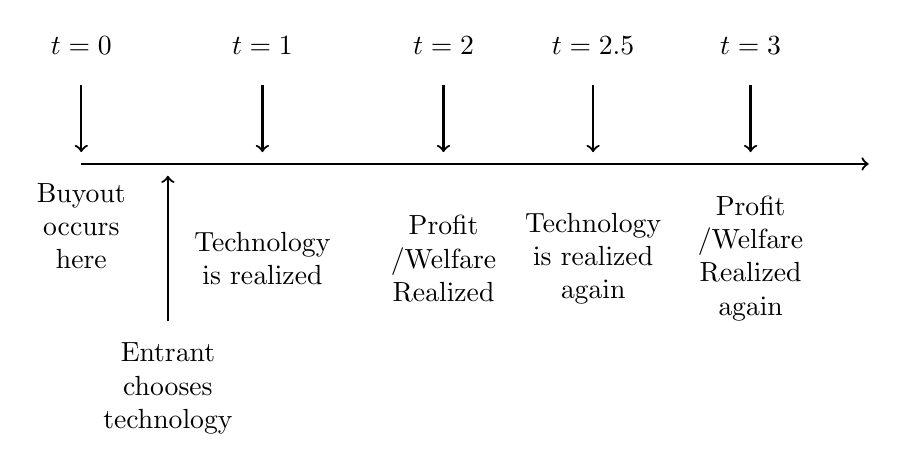
\begin{tikzpicture}[scale=1]
\node[align=center] at (0,1.5) {$t = 0$};
\draw [thick,->] (0,1) -- (0,0.15);
\node[align=center] at (0,-.7) {\\ Buyout \\ occurs\\ here};
%%%%%%%%%%%%%%%%
\node[align=center] at (2.3,1.5) {$t = 1$};
\draw [thick,->] (2.3,1) -- (2.3,0.15);
\node[align=center] at (2.3,-1.2) 
{Technology\\ is realized };
%%%%%%%%%%%%%%%%
\draw [thick,->] (1.1,-2) -- (1.1,-0.15);
\node[align=center] at (1.1,-2.85) {Entrant \\chooses\\ technology };
%%%%%%%%%%%%%%%%
\node[align=center] at (4.6,1.5) {$t = 2$};
\node[align=center] at (4.6,-1.2) {Profit\\ /Welfare\\ Realized };
\draw [thick,->] (4.6,1) -- (4.6,0.15);
%%%%%%%%%%%%%%%%
\node[align=center] at (6.5,1.5) {$t = 2.5$};
\node[align=center] at (6.5,-1.2) {Technology \\ is realized \\ again};
\draw [thick,->] (6.5,1) -- (6.5,0.15);
%%%%%%%%%%%%%%%%
\node[align=center] at (8.5,1.5) {$t = 3$};
\node[align=center] at (8.5,-1.2) {Profit\\ /Welfare\\ Realized\\ again};
\draw [thick,->] (8.5,1) -- (8.5,0.15);
%%%%%%%%%%%%%%%%
%%%%%%%%%%%%%%%%
\draw [thick,->] (0,0) -- (10,0);
\end{tikzpicture}

The analysis in this case is straightforward, we need only calculate the difference in profits in the case with the radical innovation and the sequential innovation. 

\begin{proposition}
If the buyouts are ex-ante, the decision criteria for the radical innovation to be chosen by the incumbent is: 
\begin{equation*}
\frac{3-\sqrt{5}}{2}<q^*
\end{equation*}
\end{proposition}

\begin{proof}
We need only set 
\begin{align*}
\Pi_{r}^m >\Pi_{s}^m \\
\pi_i(c_i,c_e) (1-q) (2-q)+\pi_i(c_{i2},c_e) q (3-q)>\pi_i(c_i,c_e) +  \pi_i(c_{i2},c_e) 
\end{align*}
\end{proof}

This is intuitive because, if the radical innovation has a high enough probability of being achieved, the incumbent will opt for it. Note that the ex-ante case is identical for both Cournot and Bertrand competition. If there is a reputational mechanism at work or perhaps a working relationship that already exists between the entrant and the incumbent then the ex-ante case becomes more plausible. Signaling mechanisms may also exist that enable the ex-ante buyout to occur. For instance if there is some way for the entrant to communicate why they can undertake a specific invention then this will also suffice.

\subsection{Ex-post Bertrand}
The ex-post case is simply the setup we used in the more general case. Apart from the incomplete contract justifications, it could occur because there are simply too many firms innovating and the incumbent cannot tell who has innovative capabilities before they invest. Bertrand competition reduces the distortion effect to a much simpler form, this is because in Bertrand competition only the highest technology firm makes profits. Additionally we know that the payoffs, when not the monopoly payoff, will be that the most advanced firm will price at the production cost of the second most advanced firm. Therefore $\pi_i(c_i,c_{e1})= (1-c_{e1})(c_{e1}-c_i)$ and $\pi_e(c_i,c_{e2})= (1-c_{i})(c_{i}-c_{e2})$

 

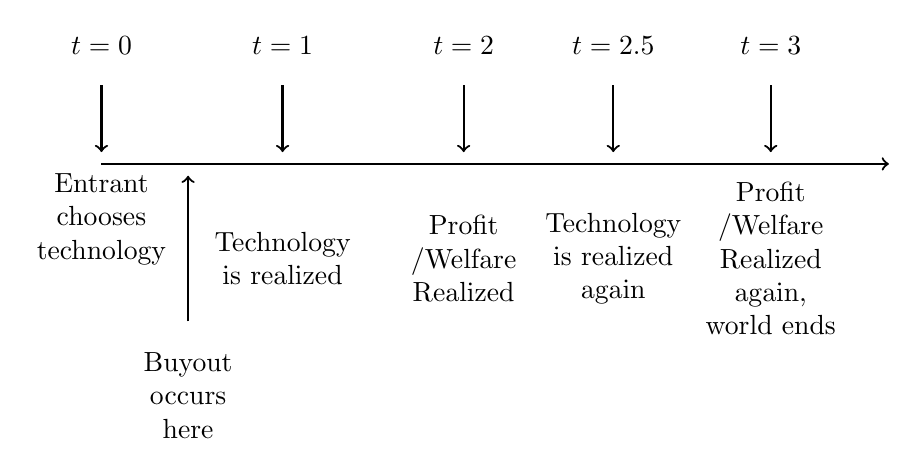
\begin{tikzpicture}[scale=1]
\node[align=center] at (0,1.5) {$t = 0$};
\draw [thick,->] (0,1) -- (0,0.15);
\node[align=center] at (0,-.7) {Entrant \\chooses\\ technology};
%%%%%%%%%%%%%%%%
\node[align=center] at (2.3,1.5) {$t = 1$};
\draw [thick,->] (2.3,1) -- (2.3,0.15);
\node[align=center] at (2.3,-1.2) {Technology\\is realized };

%%%%%%%%%%%%%%%%
\draw [thick,->] (1.1,-2) -- (1.1,-0.15);
\node[align=center] at (1.1,-2.85) { \\ Buyout \\ occurs\\ here};
%%%%%%%%%%%%%%%%
\node[align=center] at (4.6,1.5) {$t = 2$};
\node[align=center] at (4.6,-1.2) {Profit\\ /Welfare\\ Realized };
\draw [thick,->] (4.6,1) -- (4.6,0.15);
%%%%%%%%%%%%%%%%
\node[align=center] at (6.5,1.5) {$t = 2.5$};
\node[align=center] at (6.5,-1.2) {Technology \\ is realized \\ again};
\draw [thick,->] (6.5,1) -- (6.5,0.15);
%%%%%%%%%%%%%%%%
\node[align=center] at (8.5,1.5) {$t = 3$};
\node[align=center] at (8.5,-1.2) {Profit\\ /Welfare\\ Realized\\ again, \\ world ends};
\draw [thick,->] (8.5,1) -- (8.5,0.15);
%%%%%%%%%%%%%%%%
%%%%%%%%%%%%%%%%
\draw [thick,->] (0,0) -- (10,0);
\end{tikzpicture}

If the buyout is not possible the bargaining payoffs are not available for either firm. Under such conditions the entrant will simply compare the direct market payoffs of the innovation. 

\begin{proposition}
If no buyouts can occur, the entrants preferences for the radical innovation are identical to the incumbent when the buyout is ex-ante.
\end{proposition}

\begin{proof}
\begin{align*}
\Pi_{er}&> \Pi_{es}  \\
q\pi_e(c_i,c_{e2})(3-q) &>  \pi_e(c_i,c_{e2}) \\
\pi_e(c_i,c_{e2})(q(3-q)-1) &> 0
\end{align*}

\begin{equation*}
q> \frac{3-\sqrt{5}}{2}=q^b
\end{equation*}

Notice that, $q^b=q^*$, therefore the preferences are identical. 
\end{proof}

In other words, no distortion effect occurs if there are no buyouts. The result is not necessarily intuitive because the profits being compared are not of the same type. That is, the incumbents profits are monopoly profits whilst the entrants profits are competitive. Nevertheless since the absolute value of the gain does not play a role but only the relative gain does, this drives the result.
We now proceed to compare the choice between the radical and sequential innovation when buyouts are allowed.

\begin{proposition}
\label{higherq}
If buyouts are possible, then the q required for the radical innovation to be pursued will be higher than $q^b=q^*$. 
\end{proposition}

\begin{proof}
If buyouts are allowed, the radical innovation will be pursued if:
\begin{align*}
&B_{er}(\omega)>B_{es}(\omega) \\
\rightarrow q \pi_{e}(c_{i},c_{e2})(3-q)&(1-\omega)
+ \omega q 
\pi_{i}(c_{i2},c_{e}) (3-q) \\
> \pi_{e}(c_{i},c_{e2})&(1-\omega)+ \omega (\pi_{i}(c_{i},c_{e}) +  \pi_{i}(c_{i2},c_{e}) - \pi_{i}(c_{i},c_{e1}) ) \\
\leftrightarrow \pi_{e}(c_{i},c_{e2})(q(3-q)-1)&(1-\omega)
+ \omega \pi_{i}(c_{i2},c_{e}) (q(3-q)-1)-\omega(\pi_{i}(c_{i},c_{e})- \pi_{i}(c_{i},c_{e1})) 
> 0 \\
\end{align*}

Note that the third term is negative because $\pi_{i}(c_{i},c_{e})$ is a monopoly profit whilst  $\pi_{i}(c_{i2},c_{e})$ is a competitive profit. This implies that unlike before for the inequality to be satisfied, q must not only be large enough to make the expressions it interacts with positive but it must also be large enough to overcome the third term.
\end{proof}

Note that this is just a special case of proposition \ref{excessincentive}. But it serves to illustrate how the expression simplifies due to the Bertrand assumptions. Bertrand competition the preference shift is entirely due to the difference in profit of the incumbent between the default profit and the profit against an entrant with intermediate cost, in other words the externality,   $\omega(\pi_i(c_i,c_e)- \pi_i(c_i,c_{e1})) $. The fact that the entrant can bargain on the externality is is the driving factor behind this result. 



%\begin{proposition}
%If both firms cost the same, the ability to buyout can only shift the %incentive towards the sequential innovation. 
%\end{proposition}

%\begin{proof}
%We need only use the expression from the previous proposition and compute if

%\begin{align*}
%B_{ER}-\overline{\Pi}_{ER}-B_{ES}+\overline{\Pi}_{ES} =  \\
%=\omega q 
%\left(
%\pi_{i2} (3-q)
%-\pi_{e2}(3-q)
%\right)-\omega (\pi_{i} +  \pi_{i2} - \pi_{i1}-\pi_{e2} )  > 0 \\
%=\omega  
%\left(
%\pi_{i2} (3q-q^2-1)
%-\pi_{e2}(3q-q^2-1)-\pi_{i}+\pi_{i1}
%\right)  > 0 \\
%=
%\pi_{i2} (3q-q^2-1)
%-\pi_{e2}(3q-q^2-1)-\pi_{i}+\pi_{i1}  > 0 
%\end{align*}
%Which is always true since the first term is a monopoly profit whilst the %second term is a competitive profit. 

%Since the change in incentives is larger for the radical innovation than for %the sequential innovation it implies that 
%\end{proof}




%%\section{Consumer surplus}

%%There four possible consumer surplus outcomes. The two monopoly outcomes, where the incumbent has the default or the highest technology, $S_I$ and $S_{I2}$, respectively. Or the two competitive outcomes, where the incumbent must set a price when the entrant has an intermediate technology and when the entrant has the highest technology, $S_{I1}$ and $S_{E}$ respectively. 

%%A reminder that the social surplus is found by computing:

%%\begin{align*}
%%S_I =  \frac{(1-c_i)^2}{8};  ~~
%%S_{I2}=  \frac{(1-c_{i2})^2}{8}; ~~
%%S_{I1} = \frac{(1-c_{i1})^2}{2};~~
%%S_{E} =  \frac{(1-c_i)^2}{2}
%%\end{align*}

%%The total consumer surplus in both time periods if there if no investment takes place is simply: 

%%\begin{align*}
%%CS=\frac{(1- p)(1-p)}{2}+\frac{(1-p)(1-p)}{2} \\
%%= \frac{(1-c_i)^2}{4} \\
%%=2 S_{I}
%%\end{align*}

%%Consumer surplus if entrant chooses sequential innovation but there is no buyout:

%%\begin{align*}
%%\overline{CS}_{S} = 
%%S_{I1}
%%+
%%S_{E}\\
%%\end{align*}

%%If there is a buyout with the first technology being pursued then consumer surplus is simply. 

%%\begin{align*}
%%CS_{S} = 
%%S_{I}
%%+
%%S_{I2}\\
%%\end{align*}

%%If no buyout occurs and the radical innovation is pursued then:

%%\begin{align*}
%%\overline{CS}_{R} =(1-q)\left(
%%S_I
%%+ \left( q S_{E}
%%+(1-q) S_I
%%\right)
%%\right)
%%+
%%q S_E \\
%%=\frac{(1-c_i)^2}{8}\left(2+9q%%-3q^2
%%\right) \\ 
%%= S_i \left(2+9q-3q^2
%%\right)
%%\end{align*}

%%If a buyout occurs with the radical innovation then the respective total surplus is: 

%%\begin{align*}
%%CS_{R} = 2 q S_{I2}+(1-q)(S_{I}+(qS_{I2}+(1-q)S_{I})) \\
%%= (3-q) q S_{I2}
%%+(1-q)(2-q) S_{I}
%%\end{align*}



%%\begin{proposition}
%%The consumers prefer the radical innovation if there is no buyout if: 
%\begin{equation*}
%q > \frac{9 S_I - \sqrt{3 S_I} \sqrt{35  S_I-4 (S_{I1}
%+
%S_{E})
%}}{6 S_I}
%\end{equation*}
%\end{proposition}

%\begin{proof}
%\begin{align*}
%\overline{CS}_{R}>\overline{CS}_{S} \\
%S_I \left( 2+9q-3q^2
%\right) >  S_{I1}
%+ S_{E} \\
%\rightarrow q > \frac{9 S_I \pm \sqrt{3} \sqrt{S_I \left(35 S_I-4 (S_{I1}
%+
%S_{E})
% \right)}}{6  S_I} \\
%\text{The positive solution %exceeds 1, therefore:} \\
%q > \frac{9 S_I - \sqrt{3} %\sqrt{S_I \left(35 S_I-4 (S_{I1}
%+
%S_{E})
% \right)}}{6  S_I}
%\end{align*}
%\end{proof}

%\begin{proposition}
%A minimum condition for it to be possible for consumers to be indifferent between radical and sequential innovation is. 
%\end{proposition}
%
%\begin{corollary}
%If consumer do not discount %this expression simplifies to: 
%\begin{align*}
%q > \frac{9 S_I - \sqrt{3 S_I} %\sqrt{ 35 S_I-4 (S_{I1}
%+ S_{E})
% }}{6 S_I} \\
%q >  \frac{3}{2}- \frac{\sqrt{3 } \sqrt{ 35 S_I-4 (S_{I1}
%+ S_{E})
% }}{6 \sqrt{S_I}} \\ 
%\text{We compute the term inside the parenthesis:} \\
%\sqrt{ 35 S_I-4 (S_{I1}
%+ S_{E})  } \\
%\sqrt{ 35\left( \frac{(1-c_{i})^2}{8}\right) -4 \left( \frac{(1-c_{i1})^2}{2}
%+ \frac{(1-c_i)^2}{2} \right) } \\
%\sqrt{ \frac{70}{16}\left( (1-c_{i})^2\right) -\frac{32}{16} \left( (1-c_{i1})^2
%+ (1-c_i)^2\right) } \\
%\frac{1}{4} \sqrt{ 70 (1-c_{i})^2 -32  (1-c_{i1})^2
%- 32 (1-c_i)^2 } \\
%\frac{1}{4} \sqrt{ 38 (1-c_{i})^2 -64  (1-c_{i1})^2 } \\
%\end{align*}
%\end{corollary}

%The maximum gap between the intermediate cost and the default cost so that there exist values of q for which a

%If we set 


%\begin{align*}
%\frac{3}{2}- \frac{\sqrt{3 } \sqrt{ 35 S_I-4 (S_{I1}
%+ S_{E})
% }}{6 \sqrt{S_I}} 
%\end{align*}

%We use this simplification the RHS above to see that the minimum difference between the two so that it is possible to prefer the radical innovation is:


%Since this is a Bertrand paradigm it is trivial to see that if both projects are profitable, from the consumer stand point it is preferred that there not be a buyout. This stems from the simple fact that the monopoly outcome decreases both the number of consumers and increases the price for those who end up consuming. 

%However because there is a cost to the investment, consumers may prefer the buyout to exist if both projects are unprofitable. This is simple to see, we need only note that if there is no entrant there is guaranteed monopoly with cost $c_i$. However if the buyout incites the entrant to enter and gets bought out, the new optimal monopoly price using $c_{I2}$ will be lower than the previous one. Note that if consumers prefer there to be a buyout policy this is sufficient to see that the buyout policy is pareto improving. 

\subsubsection{When does the buyout option help the incumbent?}

We now return to the case where we consider the point of view of the incumbent. By looking at the preferences of the incumbent we can also derive a willingness to lobby. That is, if the incumbent loses from the ability to buyout because the competitive effect is larger than the potential technology boost. It is trivial to note that the incumbent does not have a willingness to lobby if the option to buyout does not change the preferences of the entrant. The incumbent will prefer to the buyouts to exist as a function of his own bargaining power, $1-\omega$. We again look at the special case of the Bertrand competition with parameters $T=t_2=2,t_1=1$. In what corresponds to case \ref{case:decision} in the general section, the conditions collapses to the following. 

\begin{align*}
B_{is}(\omega)&>2 \pi_i(c_i,c_e) \\
& \leftrightarrow -\omega(\pi_i(c_i,c_{e})- \pi_i(c_i,c_{i1})) 
%%%%%%%%%%%%%%%%%%%%%%%%%%%%%%%%%%%%%
+(1-\omega)(\pi_i(c_{i2},c_e)-\pi_e(c_{i},c_{e2})) >0 \\
%%%%%%%%%%%%%%%%%%%%%%%%%%%%%%%%%%%%%
1-\omega &> \frac{\pi_i(c_i,c_{e})- \pi_i(c_i,c_{i1})}{\pi_i(c_i,c_{e})- \pi_i(c_i,c_{i1})+\pi_i(c_{i2},c_e)-\pi_e(c_{i},c_{e2})}
\\
%%%%%%%%%%%%%%%%%%%%%%%%%%%%%%%%%%%%%
B_{ir}(\omega)&>2 \pi_i(c_i,c_e) \\
%%%%%%%%%%%%%%%%%%%%%%%%%%%%%%%%%%%%%
& \leftrightarrow ((1-\omega)(\pi_{i}(c_{i2},c_{e})-\pi_{e}(c_{i},c_{e2}))-\pi_i(c_i,c_e)) q(3-q)>0 \\
%%%%%%%%%%%%%%%%%%%%%%%%%%%%%%%%%%%%%
1-\omega&>\frac{\pi_i(c_i,c_e)}{\pi_i(c_{i2},c_e)-\pi_i(c_{i},c_{e2})}
%%%%%%%%%%%%%%%%%%%%%%%%%%%%%%%%%%%%%
\end{align*}

The first result is the outcome if the buyout incentivizes the entrant to innovate with the sequential technology when the entrant would have otherwise not innovated at all. The bargaining power must be greater than the ratio of the profit loss from the externality,$\pi_i(c_i,c_{e})- \pi_i(c_i,c_{i1})$ to the profit loss from the externality and the difference in profit from what the incumbent can achieve with the best technology and what the entrant can achieve with the best technology,$\pi_i(c_{i2},c_e)-\pi_e(c_{i},c_{e2})$. 

Similarly with the radical innovation it must just be that the bargaining power of the incumbent is greater than the ratio of the default profit to the difference in profit from what the incumbent can achieve with the best technology and what the entrant can achieve with the best technology. Notice that this means that in the radical case, the willingness to lobby for buyouts is independent of the efficiency of the technology, $q$. This is because $q$ is equally harmful as it is helpful, a high $q$ increases the probability of achieving the high result but it also increases the negotiating power of the entrant by an equal amount. 

Finally we have the case where the entrant would have entered anyway but will instead pursue the sequential innovation. Since the entrant would have entered anyway but the only thing that has changed is the choice of innovation this is simply the difference in payoff between bargaining for the sequential technology and competing with the radical technology. 

\begin{align*}
&B_{is}(\omega)>\Pi_{ir} \\
%%%%%%%%%%%%%%%%%%%%%%%%%%%%%%%%%%%%%%
\leftrightarrow &\pi_i(c_i,c_e)(q(3-q) -\omega) 
%%%%%%%%%%%%%%%%%%%%%%%%%%%%%%%%%%%%%%
+\omega \pi_i(c_i,c_{i1}) 
%%%%%%%%%%%%%%%%%%%%%%%%%%%%%%%%%%%%%%
 +(1-\omega)(\pi_i(c_{i2},c_e)-\pi_e(c_{i},c_{e2})) 
%%%%%%%%%%%%%%%%%%%%%%%%%%%%%%%%%%%%%%
> 0 \\
%%%%%%%%%%%%%%%%%%%%%%%%%%%%%%%%%%%%%%
\leftrightarrow &
(1-\omega)> \frac{\pi_i(c_i,c_e)(1-q(3-q))-\pi_i(c_i,c_{i1})}{\pi_i(c_i,c_e)-\pi_i(c_i,c_{i1})+\pi_i(c_{i2},c_e)-\pi_e(c_{i},c_{e2})}  
\end{align*}

Notice here that $q$ does enter into the equation. The higher $q$ is the higher is the willingness to lobby and the lower the required barganing power for the incumbent to wish to lobby. 

\subsection{Ex-Post Cournot}

We will not detail the calculations the Cournot, our main purpose for this section is to show that the distortion of buyouts in Cournot is lower than in Bertrand. The payoffs of the entrant and incumbent in Cournot, with the same demand function as before, $D(q)=1-q$ are given by:

\begin{align*}
\pi_{e}(c_i,c_{e1}) &= \left(\frac{1-2 c_{e1}+c_{i}}{3}  \right)^2;
\pi_{e}(c_i,c_{e2}) = \left(\frac{1-2 c_{e2}+c_{i}}{3}  \right)^2; \\
\pi_{i}(c_i,c_{e1}) &= \left(\frac{1+ c_{i1}-2c_{i}}{3}  \right)^2;
\pi_{i}(c_i,c_{e2}) = \left(\frac{1+ c_{i2}-2c_{i}}{3}  \right)^2 \\
\end{align*}


If $c_i-c_{e1}=c_{e2}-c_i$ this would would imply the simplification that $\pi_{e}(c_i,c_{e1})=\pi_{i}(c_{i},c_{i2})$ and $\pi_{e}(c_i,c_{e2})=\pi_{i}(c_{i},c_{i1})$, this entailment would also hold in the case of Bertrand competition, $\pi_{e2}^{c}=\pi_{i2}^{c}$ and $\pi_{e1}^{c}=\pi_{i1}^{c}$. As before we assume the initial profit is a monopoly profit. The first result is that the sequential innovation is pursued more often in than in Bertrand.

\begin{proposition}
Without buyouts, if the radical innovation is preferred in Cournot competition, it is also preferred in Bertrand. 
\end{proposition}

\begin{proof}
\begin{align*}
\Pi_{er}&>\Pi_{es} \\
%%%%%%%%%%%%%%%%%%%%%%%%%%%%%%%%%%%%
q \pi_{e}(c_i,c_{e2}) (3-q) &> \pi_{e}(c_i,c_{e1})+\pi_{e}(c_i,c_{e2}) \\
%%%%%%%%%%%%%%%%%%%%%%%%%%%%%%%%%%%%
q&> 
 \frac{3}{2}-\frac{ \sqrt{5 \pi_{e}(c_i,c_{e2})-4 \pi_{e}(c_i,c_{e1})}}{2 \sqrt{\pi_{e}(c_i,c_{e2})}}=q^{c}
\end{align*}

We need only see that $q^{c}>q^{b}$. To do so we can notice that $\frac{\partial q^c}{\partial \pi_{e}(c_i,c_{e1}) }$ is positive and that if $\pi_{e}(c_i,c_{e1})=0$, we are left with $q^{b}$
\end{proof}

The intuition behind this result is due to the lower advantage of being the market leader. In Cournot the entrant earns a profit even with the intermediate technology which makes the lag time between the intermediate stage and the advanced stage less important. This means the entrant requires a higher $q$ to be convinced to pursue the radical innovation.  

\begin{proposition}
If the payoff of the incumbent when the entrant has the advanced technology is the same in both Bertrand and Cournot competition, the cutoff point for the radical innovation to be pursued with buyout is lower than in Bertrand. 
\end{proposition}

\begin{proof}
\begin{align*}
\Pi_{er} + \omega NS_{r}
> \Pi_{es} + \omega NS_{s} \\
%%%%%%%%%%%%%%%%%%%%%%%%%
(q  (3-q)-1)((1-\omega)\pi_{e}(c_i,c_{e2})+\omega((\pi_{i}(c_{i2},c_{e})-\pi_{i}(c_i,c_{e1})))) \\
+(1-\omega)\pi_{e}(c_i,c_{e1})
-\omega(\pi_{i}(c_i,c_{e}) 
-\pi_{i}(c_{i},c_{e2}))>0
\end{align*} 
Note here that this expression is identical to the expression in proposition \ref{higherq} except for the extra term, $\pi_{e}(c_i,c_{e1})(1-\omega)$ which is always positive. Note however that this not entail the cuttoff point is always higher than in Bertrand, it depends on if gap between $\omega(\pi_{i}(c_i,c_{e}) 
-\pi_{i}(c_{i},c_{e2}))$ is higher than the same gap in Bertrand competition. Note that the monopoly profit,$\pi_{i}(c_i,c_{e})$ is identical in both cases. Therefore if the profit of the incumbent when the entrant has the advanced technology is identical in both Cournot and Bertrand, Cournot has a lower q for it to be pursued due to the extra positive term, $(1-\omega) \pi_e(c_i,c_{e1})$ 
\end{proof}

The buyout case has two relevant effects which are in friction. On one hand the same effect as the non-buyout case, namely that being behind is not as important to the entrant. However there is now a second effect which is that the incumbent is less harmed by being overtaken, so there is a lower willingness to buyout. Note that since $q^b<q^c$ without buyout, and $q^b>q^c$ when there is a buyout, this means the difference between the buyout and the non-buyout case is smaller in Cournot than in Bertrand. Which means that the distortion effect is lower overall for the case of Cournot. 

\section{Discussion}\label{discussion}

The intuition behind result \ref{higherq} is a consequence of the Coase theorem. The activity of the entrant can be interpreted to have an externality on the incumbent. Both the radical and sequential innovation have such an externality. However the sequential innovation has an externality with no associated direct benefit to the entrant beyond the ability to threaten the incumbent. In other words, if there was no bargaining, the entrant would be indifferent to increasing the damage done to the incumbent, it is a variable which does not enter into the decision criteria. However as soon as there is a buyout, the entrant now can negotiate on the negative externality that is being pushed on the incumbent. This incites the entrant to pursue the technology that has has this externality relatively more than before. 

The ability to blackmail has been studied in the context of the Coase theorem, \cite{Dem}. In the rancher and farmer case study, the rancher has his cows graze whilst the farmer grows crops. If we suppose that the rancher does not have to compensate the farmer for the damage done, then the farmer will be willing to pay to stop the rancher. However in such a case, if the rancher has options which are not individually attractive but are very costly to the farmer, she can use these options to extort the farmer into giving a higher payment. It is important that the rancher be able to commit to applying this costly action, otherwise if the farmer can just say no to the offer, it is not credible that the rancher will act in a costly manner. If commitment is possible, the rancher will over-commit(relative to the efficient outcome) to the option which causes harm to the farmer.

In fact this is very similar to our story here. When the entrant pursues the radical innovation there is an externality to the choice where it threatens to take away the profits of the incumbent, this is a productive action that can occur in either of the two periods. On the other hand the sequential innovation can be seen as an unproductive action followed by a productive action. This case is to be juxtaposed to a sequential innovation that would have no externality to the incumbent, this would reduce the payoff potential of the entrant if there is a buyout and be less distortionary. 

It is interesting that there are different informational requirements in the two cases. In the case of no buyouts the informational pre-requisites on the entrant are simply to know the profit potential of the project, the cost of the project, and the probability of innovating. On the other hand the ability to buyout actually has a higher burden in terms of rationality on the entrant, that is to compute the optimal decision one must know not only the potential payoffs of the project but also the revenue loss of the incumbent and the negotiating power. So while the model made abstractions from information asymmetries, it is quite clear that buyouts have a higher information burden, this could be captured merely by interpreting it as part of the cost. 

We include the details of the welfare analysis in the appendix but give some cursory details here. In general since the buyout causes a monopoly this monopoly needs to be an improvement from what would occur otherwise, there are only two cases to consider. One alternative a less efficient monopoly, that is a monopoly with the high cost of production, this case occurs if without the buyout the entrant would not enter. Relative to this less efficient monopoly, the buyout can only improve the situation with a more efficient monopoly. The second alternative could be that the entrant would have pursued the innovation anyway, but the effect of the entrant on the market is less important and the more efficient monopoly gives a higher welfare. However this second case is not achievable in the modes of competition used here.

It is perhaps also interesting to ask which of the projects maximize welfare. The answer is a bit complex, the welfare maximizing choice with buyouts is the same as the profit maximizing choice without buyouts(see appendix). Since we have established that the choice of the firm in the ex-ante case pursue the radical innovation more often, this implies that whenever there is a preference reversal without affecting the decision entry, this reduces welfare. The reason this occurs is because the negative externality in the intermediate period is internalized when there is a buyout. This is consistent with coase as it implies that the efficient option is pursued either when the externality is ignored by entrant or when it is fully internalized due to the buyout.

The model predicts a number of things for industry structure. If the entrant is unknown to the incumbent until the the entrant starts to innovate, this immediately gives rise to distorting effects.  This may occur if we have an industry where innovation occurs from many small entrants, the prediction is that the small entrant will over-pursue incremental innovations because it is the best way to make their project profitable. An example of such an industry is the relationship of biotechnological firms to the pharmaceutical industry. That is, numerous small entrants who threaten the incumbent who is already firmly established. On the other hand if an industry has endogenous mechanisms so that buyouts can occur before irreversible directional investments are undertaken, such as reputational mechanisms, then that industry will have have a higher tendency to pursue radical innovations. 

The model presented is specifically about cost side innovations, the strength of the conclusions depends on the ratio of production to development cost. A high production cost is about producing the marginal unit, if this is expensive then a proportional decrease in this cost will have greater effect on competitive pressure. A high development cost implies that the creation of the product has a sunk cost in the beginning which blocks entry, if this is low then industries may more easily enter and hence there will be more interactions of the sort described in this model. A high development cost is important for the buyouts described because such a cost, like all sunk costs, cannot be used for negotiating with the incumbent. Examples of industries with a high production to development cost are established industries where the good is generally larger, for instance cars, trains, airplanes, boats or metalworks are likely to have a high cost of production without there there being a high cost to development. A simple of example of an industry where the model implies the effects will be weaker is an industry such as the information technology sector, this is because software exhibits very high development cost(programming) and a low cost to produce a unit of software.  

A rather different method of envisioning a cost side innovation is management changes. Some entrant may have some cutting edge method of managing employees that can either reduce the cost of the firm gradually or it may have some scheme were a large structural change occurs and the costs are reduced quickly. The application of the model in this case is that incumbents will buyouts will lead to the entrant over-pursuing the slow employee cost reduction technique rather than the fast and risky one.  

Another natural example of a cost side innovation is energy innovations. Perhaps rather intuitively, firms are more likely to buyout entrepreneurs who can cause damage even with an ineffective technology than firms with much better prospects for advancement but no intermediate stage. In energy this may look like firms buying out solar or wind technologies more than buying out nuclear plans.   



\section{Conclusion}


The paper presents a preference reversal within two paradigms. We find that policy levers have ambiguous effects, enabling buyouts can have both a negative and positive effects on welfare and this is not necessarily a function of the willingness to pay. Instead it is purely a function of substitutability and complementarity. Empirically, the willingness to pay of incumbents for the entrants cannot be used as a proxy for reducing rent seeking since, the willingness to pay can stem equally from substitutability and complementarity. 

We present a simple model which implies that mergers should not only be seen from a point of view of competition vs efficiency but also from the point of view of innovative convergence. When firms can buy other firms this is in essence license for firms to play correlated strategies and there is a strong incentive for firms to choose industries which are already existing without reasons having to do with industry level characteristics. As such anti-trust policy should take into account the effects buyouts on industry convergence. Specifically, for patents, if the role of the patent is to exclude other firms, then the kind of patenting will not be affected, if on the other hand the role of patenting is to be bought over by larger firms, this will favor industry convergence. The basic reasoning implies that either patents requirement should more stringent when an innovation improves on a product with an existing industry or if possible, if entrants represent a larger threat to incumbents, buyouts rules should be more demanding. . 

Finally, the model implies that there is a demand for lobbying. If we are in a paradigm where enabling buyouts create a preference reversal for the entrant and where this is not preferred by the incumbent, then this creates a willingness to pay from the incumbent which will disable buyouts. 


\newpage
\section*{Apendix 1: Welfare equations}

There are four possible consumer surplus outcomes. The two monopoly outcomes, where the incumbent has the default or the highest technology, $S_I$ and $S_{I2}$, respectively. Or the two competitive outcomes, where the incumbent must set a price when the entrant has an intermediate technology and when the entrant has the highest technology, $S_{I1}$ and $S_{E}$ respectively. 

A reminder that the social surplus is found by computing:
$\frac{1}{2}(1- p)(1-p)$. In the case of monopoly the price is simply the monopoly price in a Bertrand context. While if the outcome is competitive, the price is simply the competitors cost. The four possible  social outcomes are given below:

\begin{align*}
S(c_i, c_e) =  \frac{(1-c_i)^2}{8};  ~~
S(c_{i2}, c_e)=  \frac{(1-c_{i2})^2}{8}; ~~
S(c_{i}, c_{e1}) = \frac{(1-c_{i1})^2}{2};~~
S(c_{i}, c_{e2}) =  \frac{(1-c_i)^2}{2}
\end{align*}

Note that the consumer only prefers the buyouts if it incentives the entrant to pursue the projects. If the projects are already being pursued without the buyout then the consumer can only lose because whilst before there was some possibility of a competitive outcome, now there are only monopoly outcomes possible. From the welfare perspective the bargaining power only matters if it will change the choices of the firms. Otherwise bargaining power will be zero sum, therefore we need only look at the market profits and the social surplus of consumers to compute the welfare function. In the two cases where there is a monopoly this is either the monopoly with the default cost or the monopoly with the lower cost. We recall here that monopoly with the lower price is preferred over the monopoly with the default price for both consumers and the monopolist. These outcomes are given by:

\begin{align*}
w(c_{i}, c_{e}) &= \frac{(1-c_i)^2}{8} + \frac{(1-c_i)^2}{4}= \frac{3(1-c_i)^2}{8} \\
%%%%%%%%%%%%%%%%%%%%%%%%%%%%%%
w(c_{i2}, c_{e}) &= \frac{3(1-c_{i2})^2}{8} \\
\end{align*}

Similarly the welfare payoffs of both consumers and the firms are given simply by the competitive profits and the consumer surplus. This represents a shift from firms to the consumers. From the consumer point of view it is preferred that the entrant be the market leader because the price will necessarily be lower. However this does not neccesarily mean that the entrant will have less profits than the competitive case where the incumbent is ahead. 

\begin{align*}
%%%%%%%%%%%%%%%%%%%%%%%%%%%%%%
w(c_{i}, c_{e1}) &= \frac{(1-c_{i1})^2}{2} + (1-c_{i1})(c_{i1}-c_i)= \frac{(1-c_{i1})}{2} 
\left(
(1-c_{i1})+2(c_{i1}-c_i )
\right) \\
%%%%%%%%%%%%%%%%%%%%%%%%%%%%%%
w(c_{i}, c_{e2}) &= \frac{(1-c_{i})}{2} 
\left(
(1-c_{i})+2(c_{i}-c_{i2} )
\right) \\
\end{align*}

Something to note here is that while clearly if we compare the monopoly cases we have the relationship, $w(c_{i}, c_{e})<w(c_{i2}, c_{e})$, that is the monopoly outcome with the lower price is better for both consumers and the firms. However, no analogous relationship exists between $w(c_{i}, c_{e2})$ and $w(c_{i}, c_{e1})$. If the gap $c_i-c_{i2}$ and $c_{i1}-c_{i}$ are equal then we have the relationship, $w(c_{i}, c_{e2})>w(c_{i}, c_{e1})$. This is for the same reason as for the monopolist outcome, the price is lower without the profits being lower, therefore a net gain for consumers. 

Before proceeding to analyze the innovations effect on welfare, we note that the welfare without the innovation is simply:

\begin{equation*}
w(c_{i}, c_{e})+w(c_{i}, c_{e}) = \frac{3(1-c_i)^2}{4}
\end{equation*}

\subsection{Sequential}

In the sequential innovation case with no buyout, in the firs time period there will be the competitive outcome with the incumbent ahead and in the second time period the entrant will be ahead with another competitive outcome. Necessarily the price will decrease, therefore for the consumers there will be an increase in surplus in the second time period. 

\begin{align*}
\overline{W}_{S} = w(c_{i}, c_{e1})
+
w(c_{i}, c_{e2})
&=
\frac{1}{2}
\left(
(1-c_{i1})
\left(
(1-c_{i1})+2(c_{i1}-c_i )
\right)
+
(1-c_{i})
\left(
(1-c_{i})+2(c_{i}-c_{i2} )
\right) 
\right)
\\
&=1-\frac{c_{i1}^2}{2}+c_{i1} c_{i}-\frac{c_{i}^2}{2}-c_{i} (1-c_{i2})-c_{i2} \\
&=1-\frac{c_{i1}^2}{2}-\frac{c_{i}^2}{2}-c_{i} (1-c_{i2}-c_{i1})-c_{i2}
\\
\end{align*}

When the buyout occurs there is always a monopoly. So the consumers will simply have to deal with the default monopoly in the first period and with the lower cost monopoly in the second period. 

\begin{equation}
W_S = w(c_{i}, c_{e}) +  w(c_{i2}, c_{e})= \frac{3}{8}
\left(
(1-c_i)^2+(1-c_{i2})^2
\right)
\end{equation}


\subsection{Radical}

Welfare when the radical innovation is pursued and there is no buyout is similarly given by: 

\begin{align*}
\overline{W}_R &= q2w(c_{i}, c_{e2})
+(1-q)(w(c_{i}, c_{e})+(1-q)w(c_{i}, c_{e})+qw(c_{i}, c_{e2})) \\
&= q w(c_{i}, c_{e2})(3-q ) 
+(1-q)w(c_{i}, c_{e})(2-q)  \\
&=\frac{1}{8} (1-c_{i}) \left(6-c_{i} \left(7 q^2-21 q+6\right)-(1-8 c_{i2}) q^2-3 (8 c_{i2}-1) q\right)
\end{align*}

If buyouts do occur and we are in the monopoly paradigm, the consumers are always in facin high prices but have a preference for the innovation to occur, the welfare when there are buyouts is given by the expression:

\begin{align*}
W_R &= q w(c_{i2}, c_{e})(3-q )
+(1-q)w_{m1}(2-q)  \\
&= \frac{3}{8} \left((c_i-1)^2 (2-q) (1-q)+(c_{i2}-1)^2 (3-q) q\right) \\
\end{align*}

\section*{Appendix 2: Welfare results}

\begin{proposition}\label{propwelfare}
The welfare maximizing choice in the case of buyouts is identical to the entrant's optimal choice in the case of no buyout and the incumbents ex-ante choice. 
\end{proposition}

\subsection{Proof of proposition \ref{propwelfare}}

\begin{proof} \label{buyoutnobuyout}
\begin{align*}
W_R&> W_S \\
q w(c_{i2}, c_{e})(3-q )
+(1-q)w(c_{i}, c_{e})(2-q) &> w(c_{i}, c_{e}) + w(c_{i2}, c_{e}) \\
 w(c_{i2}, c_{e})(q(3-q) -1)
+w(c_{i}, c_{e})((1-q)(2-q)-1)  &> 0 \\
w(c_{i2}, c_{e})(3q-q^2-1)+w(c_{i}, c_{e})(1-3q+q^2)&>0 \\
 w(c_{i2}, c_{e})(3q-q^2-1)-w(c_{i}, c_{e})(3q-q^2-1) &>0 
\end{align*}

If the costs are the same, then radical will be preferred if:

\begin{align}
q> \frac{3-\sqrt{5}}{2}
\end{align}

Which is identical to the cutoff point for the entrant to prefer the radical innovation. 

\end{proof}

In proposition \ref{propwelfare} we look for the criterion under which welfare is maximized when \textbf{ buyouts occur} and show that they are identical to the profit maximizing criterion of the entrant when \textbf{buyouts do not occur} and the ex-ante case. To state this another way, if absent a buyout, the entrant chooses the radical innovation, then, if there are buyouts, the welfare maximizing choice is also the radical innovation. 

\begin{proposition}
\label{welfare1}
A necessary(but not sufficient) condition for the radical innovation to be welfare maximizing is that $w(c_{i}, c_{e2})+w(c_{i}, c_{e1})-2 w(c_{i}, c_{e}) > 0 $. 
Similarly for it to be possible that sequential innovation is welfare maximizing it must be that: 
$w(c_{i}, c_{e1})-w(c_{i}, c_{e2}) > 0$
\end{proposition}


\begin{proof}\label{proofofwelfare1}

\begin{align*}
\overline{W}_R>\overline{W}_S& \\
 q w(c_{i}, c_{e2})(3-q ) 
+(1-q)w(c_{i}, c_{e})(2-q)  
>
w(c_{i}, c_{e1})
+
w(c_{i}, c_{e2})&  \\
w(c_{i}, c_{e2})(3q-q^2-1 ) 
+w(c_{i}, c_{e})(2-3q+q^2) -w(c_{i}, c_{e1}) 
&>
0
\\
q^2(w(c_{i}, c_{e})-w(c_{i}, c_{e2}))
-3q(w(c_{i}, c_{e})-w(c_{i}, c_{e2}))
-w(c_{i}, c_{e2}) 
+2 w(c_{i}, c_{e}) -w(c_{i}, c_{e1})
\end{align*}

\begin{align*}
\rightarrow q &> \frac{3}{2} - \frac{  \sqrt{ w(c_{i}, c_{e})-5w(c_{i}, c_{e2})+4(w(c_{i}, c_{e1}))}}{2\sqrt{(w(c_{i}, c_{e})-w(c_{i}, c_{e2}))}}
\end{align*}

\begin{align*}
\text{So the bound for the expression to be smaller than 1 is:} \\
\frac{  \sqrt{ w(c_{i}, c_{e})-5w(c_{i}, c_{e2})+4(w(c_{i}, c_{e1}))}}{\sqrt{(w(c_{i}, c_{e})-w(c_{i}, c_{e2}))}}  &> 1 \\
 w(c_{i}, c_{e})-5w(c_{i}, c_{e2})+4(w(c_{i}, c_{e1})) & > (w(c_{i}, c_{e})-w(c_{i}, c_{e2})) \\
w(c_{i}, c_{e1})-w(c_{i}, c_{e2})  &> 0 \\
\text{Similarly for the expression to be larger than 0 we must have:} \\
\frac{  \sqrt{ w(c_{i}, c_{e})-5w(c_{i}, c_{e2})+4(w(c_{i}, c_{e1}))}}{2\sqrt{(w(c_{i}, c_{e})-w(c_{i}, c_{e2}))}} &< \frac{3}{2} \\
 w(c_{i}, c_{e})-5w(c_{i}, c_{e2})+4(w(c_{i}, c_{e1})) > 9(w(c_{i}, c_{e})-w(c_{i}, c_{e2})) \\
 4(w(c_{i}, c_{e2})+w(c_{i}, c_{e1}))-8 w(c_{i}, c_{e}) &< 0 \\
 w(c_{i}, c_{e2})+w(c_{i}, c_{e1})-2 w(c_{i}, c_{e}) &< 0
\end{align*}
\end{proof}


